\documentclass{article}
\usepackage{graphicx}
\usepackage{tikz}
\usetikzlibrary{arrows.meta} 
\usepackage{pgfgantt}
\usetikzlibrary{shapes,arrows}
\usetikzlibrary{matrix,calc,shapes}
\usepackage{amsmath, amssymb}
\begin{document}


$$
\binom{n}{i} 
$$

\begin{tikzpicture}
\draw (0,0) -- (1,2);
\end{tikzpicture}



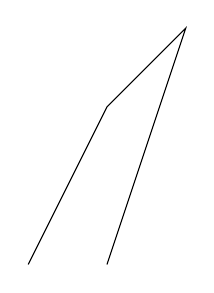
\begin{tikzpicture}
\draw (0,0) -- (1,2) -- (2,3) -- (1,0);
\end{tikzpicture}



\begin{tikzpicture}
\draw (0,0) -- (1,2) -- (2,3) -- (1,0);
\draw (3,0) -- (1.5,0.5);
\end{tikzpicture}




\begin{tikzpicture}[scale=3]
\draw (0,0) -- (1,1);
\end{tikzpicture}




\begin{tikzpicture}
\draw [->] (0,0) -- (2,0);
\draw [<-] (0, -0.5) -- (2,-0.5);
\draw [|->] (0,-1) -- (2,-1);
\end{tikzpicture}




\begin{tikzpicture}
\draw [<->] (0,2) -- (0,0) -- (3,0);
\end{tikzpicture}





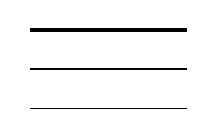
\begin{tikzpicture}
\draw [ultra thick] (0,1) -- (2,1);
\draw [thick] (0,0.5) -- (2,0.5);
\draw [thin] (0,0) -- (2,0);
\end{tikzpicture}






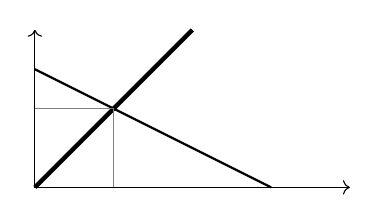
\begin{tikzpicture}
\draw [<->] (0,2) -- (0,0) -- (4,0);
\draw [thick] (0,1.5) -- (3,0);
\draw [ultra thick] (0,0) -- (2,2);
\draw [help lines] (1,0) -- (1,1) -- (0,1);
\end{tikzpicture}







\begin{tikzpicture}
\draw [line width=12] (0,0) -- (2,0);
\draw [line width=0.2cm] (4,.75) -- (5,.25);
\end{tikzpicture}







\begin{tikzpicture}
\draw [dashed, ultra thick] (0,1) -- (2,1);
\draw [dashed] (0, 0.5) -- (2,0.5);
\draw [dotted] (0,0) -- (2,0);
\end{tikzpicture}






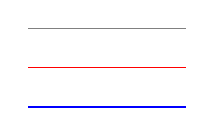
\begin{tikzpicture}
\draw [gray] (0,1) -- (2,1);
\draw [red] (0, 0.5) -- (2,0.5);
\draw [blue] (0,0) -- (2,0);
\end{tikzpicture}






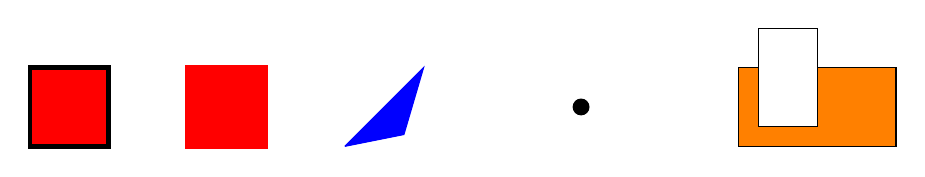
\begin{tikzpicture}
\draw [fill=red,ultra thick] (0,0) rectangle (1,1);
\draw [fill=red,ultra thick,red] (2,0) rectangle (3,1);
\draw [blue, fill=blue] (4,0) -- (5,1) -- (4.75,0.15) -- (4,0);
\draw [fill] (7,0.5) circle [radius=0.1];
\draw [fill=orange] (9,0) rectangle (11,1);
\draw [fill=white] (9.25,0.25) rectangle (10,1.5);
\end{tikzpicture}







\begin{tikzpicture}
\draw [ultra thick] (0,0) to [out=87,in=150] (1,1) -- (.85,.15) -- (0,0);
\draw [ultra thick, fill=purple] (2,0) to [out=87,in=150] (3,1) -- (2.85,.15) -- (2,0);
\path [fill=purple] (4,0) to [out=87,in=150] (5,1) -- (4.85,.15) -- (4,0);
\end{tikzpicture}







\begin{tikzpicture}
\path [fill=gray] (0,0) rectangle (1.5,1);
\draw [fill=yellow] (2,0) rectangle (3.5,1);
\end{tikzpicture}





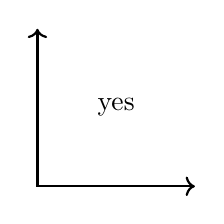
\begin{tikzpicture}
\draw [thick, <->] (0,2) -- (0,0) -- (2,0);
\node at (1,1) {yes};
\end{tikzpicture}





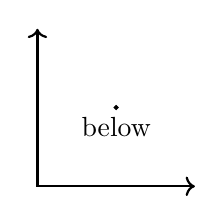
\begin{tikzpicture}
\draw [thick, <->] (0,2) -- (0,0) -- (2,0);
\draw[fill] (1,1) circle [radius=0.025];
\node [below] at (1,1) {below};
\end{tikzpicture}






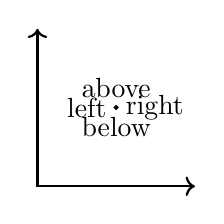
\begin{tikzpicture}
\draw [thick, <->] (0,2) -- (0,0) -- (2,0);
\draw[fill] (1,1) circle [radius=0.025];
\node [below] at (1,1) {below};
\node [above] at (1,1) {above};
\node [left] at (1,1) {left};
\node [right] at (1,1) {right};
\end{tikzpicture}






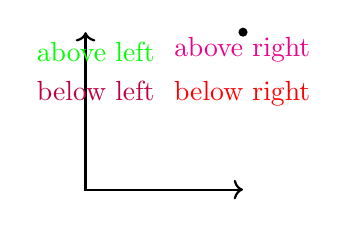
\begin{tikzpicture}[scale=2]
\draw [thick, <->] (0,1) -- (0,0) -- (1,0);
\draw[fill] (1,1) circle [radius=0.025];
\node [below right, red] at (.5,.75) {below right};
\node [above left, green] at (.5,.75) {above left};
\node [below left, purple] at (.5,.75) {below left};
\node [above right, magenta] at (.5,.75) {above right};
\end{tikzpicture}









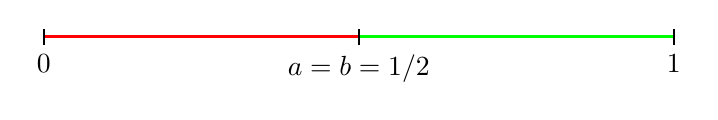
\begin{tikzpicture}[xscale=8]
\draw[-][draw=red, very thick] (0,0) -- (.5,0);
\draw[-][draw=green, very thick] (.5,0) -- (1,0);
\draw [thick] (0,-.1) node[below]{0} -- (0,0.1);
\draw [thick] (0.5,-.1) node[below]{$a=b=1/2$} -- (0.5,0.1);
\draw [thick] (1,-.1) node[below]{1} -- (1,0.1);
\end{tikzpicture}







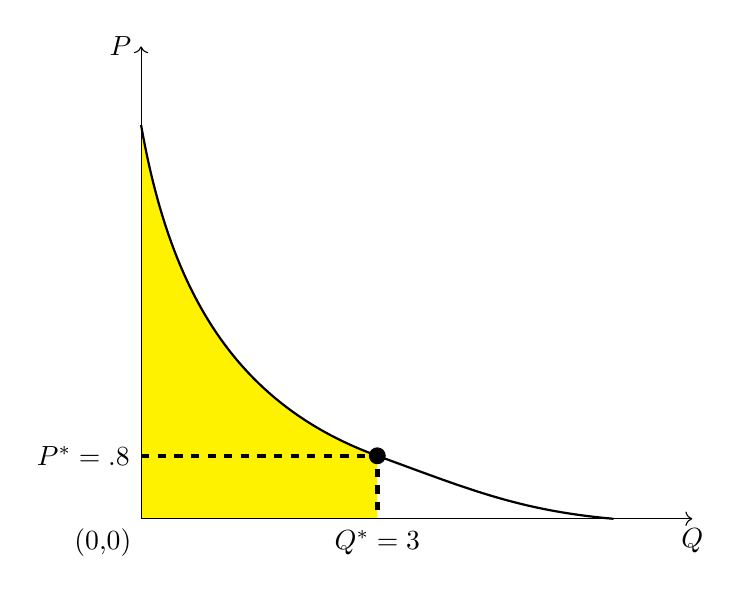
\begin{tikzpicture}
\path [fill=yellow] (0,0) -- (0,5) to [out=-80, in=160]
(3,.8) -- (3,0) -- (0,0);
\draw [<->] (0,6) node [left] {$P$} -- (0,0)
node [below left] {(0,0)} -- (7,0) node [below] {$Q$};
\draw [ultra thick, dashed] (0,.8) node [left] {$P^*=.8$} -- (3,.8)
-- (3,0) node [below] {$Q^*=3$};
\draw [fill] (3,.8) circle [radius=.1];
\draw [thick] (0,5) to [out=-80, in=160] (3,.8) to
[out=-20, in=175] (6,0);
\end{tikzpicture}







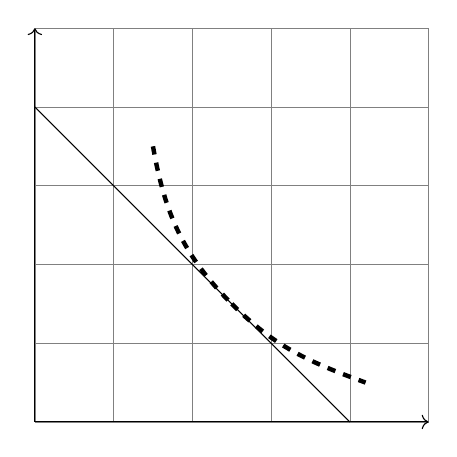
\begin{tikzpicture}
\draw [help lines] (0,0) grid (5,5);
\draw [<->] (5,0) -- (0,0) -- (0,5);
\draw (4,0) -- (0,4);
\draw[dashed,ultra thick]
(1.5,3.5) to [out=-80,in=135] (2.5,1.5);
\draw [dashed,ultra thick]
(2.5,1.5) to [out=-45,in=160] (4.2,0.5);
\end{tikzpicture}





\newpage



\begin{ganttchart}{1}{12}
\gantttitle{2011}{12} \\
\gantttitlelist{1,...,12}{1} \\
\ganttgroup{Group 1}{1}{7} \\
\ganttbar{Task 1}{1}{2} \\
\ganttlinkedbar{Task 2}{3}{7} \ganttnewline
\ganttmilestone{Milestone}{7} \ganttnewline
\ganttbar{Final Task}{8}{12}
\ganttlink{elem2}{elem3}
\ganttlink{elem3}{elem4}
\end{ganttchart}






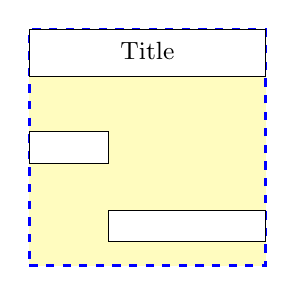
\begin{tikzpicture} % optional
\begin{ganttchart}[
canvas/.style=%
{shape=rectangle, fill=yellow!25,
draw=blue, dashed, very thick}
]{1}{6}
\gantttitle{Title}{6} \\
\ganttbar{}{1}{2} \\
\ganttbar{}{3}{6}
\end{ganttchart}
\end{tikzpicture} % optional






\begin{ganttchart}[
x unit=1cm,
y unit title=.6cm,
y unit chart=1.5cm
]{1}{6}
\gantttitle{Title 1}{6} \\
\gantttitle{Title 2}{6} \\
\ganttbar{}{1}{3} \\
\ganttbar{}{4}{6}
\end{ganttchart}







\begin{ganttchart}[
expand chart=\textwidth
]{1}{6}
\gantttitle{Title}{6} \\
\ganttbar{Bar 1}{1}{3} \\
\ganttbar{}{4}{6}
\end{ganttchart}





\begin{ganttchart}[vgrid={draw=none, dotted}]{1}{12}
\gantttitlelist{1,...,12}{1} \\
\ganttbar{}{1}{4} \\
\ganttbar{}{5}{11}
\end{ganttchart}






\begin{ganttchart}[hgrid, vgrid]{1}{6}
\gantttitle{Title 1}{3}
\gantttitle{Title 2}{3} \\
\ganttbar{}{1}{3} \ganttnewline
\ganttbar{}{2}{3}
\ganttbar{}{5}{6}
\end{ganttchart}






% Long version
\begin{ganttchart}[
vgrid,
hgrid
]{1}{12}
\gantttitle{Title}{12} \\
\ganttbar{Task 1}{1}{4} \\
\ganttbar{Task 2}{5}{6} \\
\ganttmilestone{M 1}{6} \\
\ganttbar{Task 3}{7}{11}
\ganttlink{elem0}{elem1}
\ganttlink{elem1}{elem2}
\ganttlink{elem2}{elem3}
\end{ganttchart}






% Short version
\begin{ganttchart}[
vgrid,
hgrid
]{1}{12}
\gantttitle{Title}{12} \\
\ganttbar{Task 1}{1}{4} \\
\ganttlinkedbar{Task 2}{5}{6} \\
\ganttlinkedmilestone{M 1}{6} \\
\ganttlinkedbar{Task 3}{7}{11}
\end{ganttchart}









\definecolor{foobarblue}{RGB}{0,153,255}
\definecolor{foobaryellow}{RGB}{234,187,0}
\newganttchartelement{foobar}{
foobar/.style={
shape=rectangle,
inner sep=0pt,
draw=foobarblue!50!black,
very thick,
top color=white,
bottom color=foobarblue!50
},
foobar incomplete/.style={
/pgfgantt/foobar,
draw=foobaryellow,
bottom color=foobaryellow!50
},
foobar label font=\slshape,
foobar left shift=-.1,
foobar right shift=.1
}
\begin{ganttchart}[
vgrid,
progress=today,
progress label text=\relax,
today=6
]{1}{12}
\gantttitlecalendar{day} \\[grid]
\ganttfoobar{Foobar 1}{1}{2} \\
\ganttfoobar{Foobar 2}{3}{7} \\
\ganttlinkedfoobar{Foobar 3}{9}{12}
\end{ganttchart}








\begin{ganttchart}[
vgrid,
hgrid
]{1}{12}
\gantttitle{Title}{12} \\
\ganttbar[name=b1]%
{Task 1}{1}{4} \\
\ganttbar[name=b2]%
{Task 2}{5}{7} \\
\ganttbar[name=xyz]%
{Task 3}{10}{12}
\ganttlink{b1}{b2}
\ganttlink{b2}{xyz}
\end{ganttchart}






\begin{tikzpicture}
\draw (0,0) -- (4,0);
\foreach \x/\xtext in {0,1,1.414/\sqrt{2},3.14/\pi} {
\draw (\x,0.1cm) -- (\x,-0.1cm) node[below] {$\xtext\strut$};
}
\end{tikzpicture}





\begin{tikzpicture}
\draw[->] (-5,0) -- (5,0) node[right] {$x$};
\draw[->] (0,-1) -- (0,5) node[above] {$y$};
\foreach \x in {-4,...,-1} {
\draw (\x,0.1cm) -- (\x,-0.1cm) node[below] {$\x\phantom{-}\strut$};
}
\foreach \x in {1,...,4} {
\draw (\x,0.1cm) -- (\x,-0.1cm) node[below] {$\x\strut$};
}
\foreach \y in {1,2,...,4} {
\draw (0.1cm,\y) -- (-0.1cm,\y) node[left] {$\y\strut$};
}
\node[below left=0.1cm] at (-0,0) {$0\strut$};
\begin{scope}
\clip (-5,-1) rectangle (5,5);
\draw[color=red,samples=100] plot ({\x},{\x*\x});
\end{scope}
\end{tikzpicture}




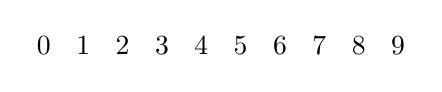
\begin{tikzpicture}
\foreach \i in {0,...,9}
\draw (\i/2,1) node {\i} ;
\end{tikzpicture}






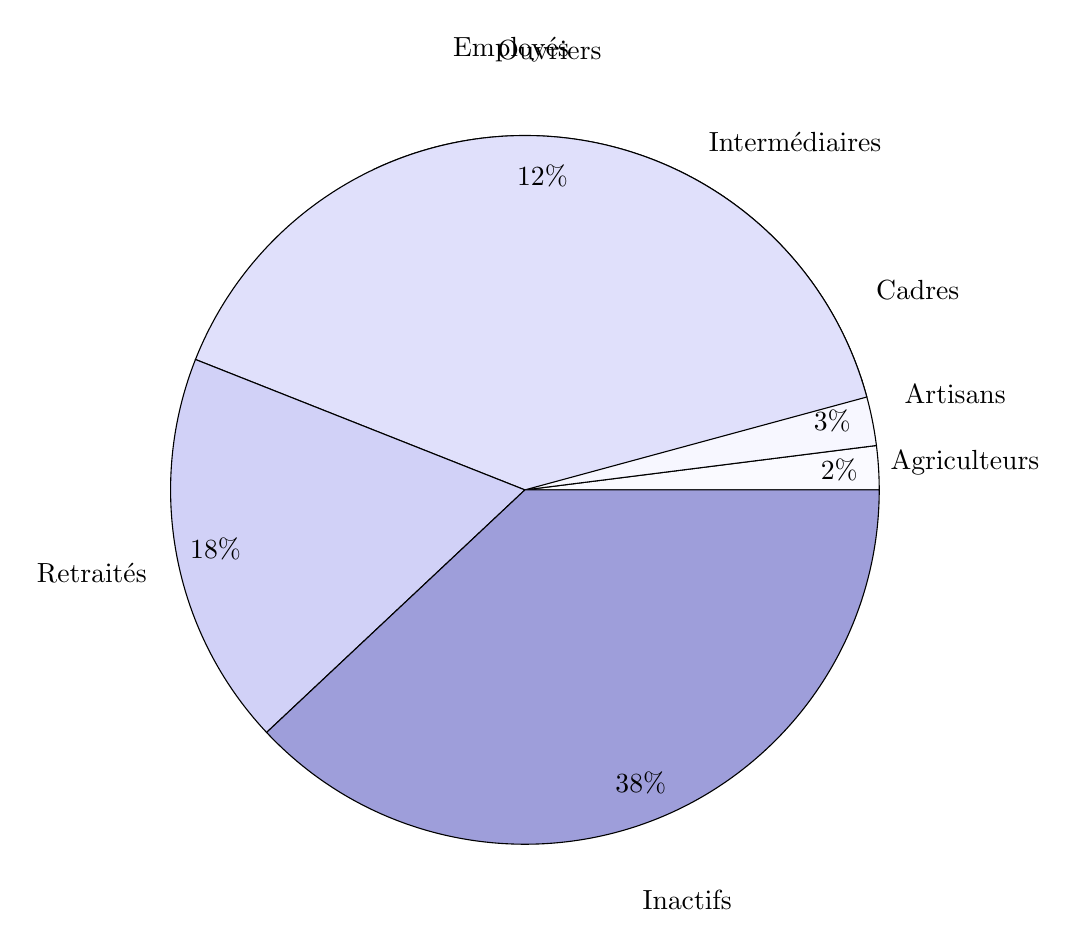
\begin{tikzpicture}
\foreach \a/\b/\p/\c in
{
0/7.2/2/Agriculteurs, 7.2/18/3/Artisans,
18/36/5/Cadres, 36/68.4/9/Intermédiaires,
68.4/115.2/13/Employés, 15.2/158.4/12/Ouvriers,
158.4/223.2/18/Retraités, 223.2/360/38/Inactifs
}
{
\draw[fill=black!\p!blue!\p]
(0,0) -- (\a:4.5) arc (\a:\b:4.5) -- cycle;
\draw ({(\a+\b)/2}:4) node {\p\%};
\draw ({(\a+\b)/2}:5.6) node {\c};
}
\end{tikzpicture}





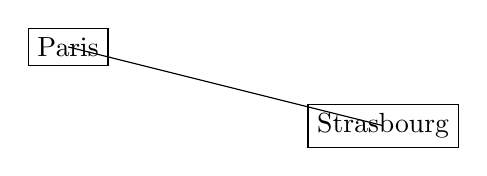
\begin{tikzpicture}
\draw (0,0)node[draw]{Paris} -- (4,-1)node[draw]{Strasbourg};
\end{tikzpicture}





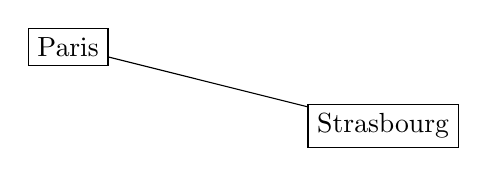
\begin{tikzpicture}
\node[draw] (P) at (0,0) {Paris};
\node[draw] (S) at (4,-1) {Strasbourg};
\draw (P) -- (S);
\end{tikzpicture}





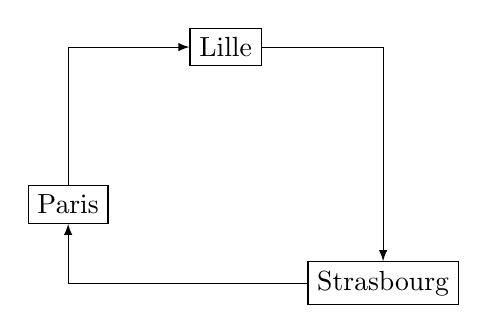
\begin{tikzpicture}
\node[draw] (P) at (0,0) {Paris};
\node[draw] (L) at (2,2) {Lille};
\node[draw] (S) at (4,-1) {Strasbourg};
\draw[->,>=latex] (P) |- (L);
\draw[->,>=latex] (L) -| (S);
\draw[->,>=latex] (S) -| (P);
\end{tikzpicture}





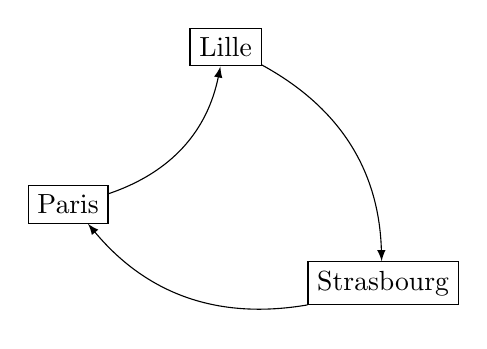
\begin{tikzpicture}
\node[draw] (P) at (0,0) {Paris};
\node[draw] (L) at (2,2) {Lille};
\node[draw] (S) at (4,-1) {Strasbourg};
\draw[->,>=latex] (P) to[bend right] (L);
\draw[->,>=latex] (L) to[bend left] (S);
\draw[->,>=latex] (S) to[bend left] (P);
\end{tikzpicture}






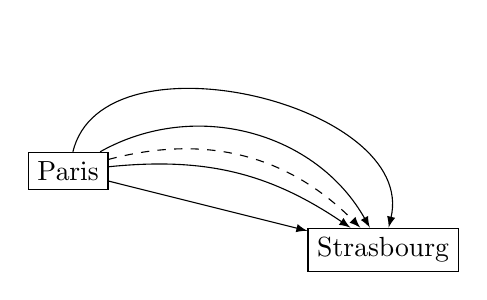
\begin{tikzpicture}
\node[draw] (P) at (0,0) {Paris};
\node[draw] (S) at (4,-1) {Strasbourg};
\draw[->,>=latex] (P) to[bend left=0] (S);
\draw[->,>=latex] (P) to[bend left=20] (S);
\draw[->,>=latex,dashed] (P) to[bend left] (S);
\draw[->,>=latex] (P) to[bend left=45] (S);
\draw[->,>=latex] (P) to[bend left=90] (S);
\end{tikzpicture}





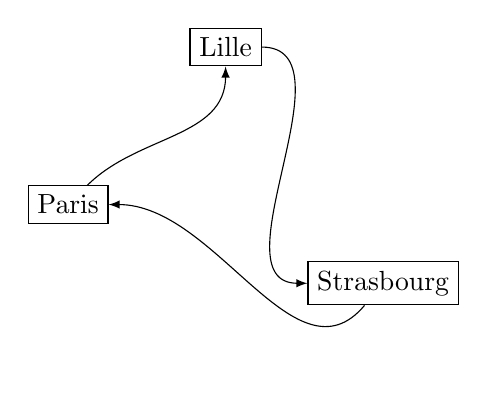
\begin{tikzpicture}
\node[draw] (P) at (0,0) {Paris};
\node[draw] (L) at (2,2) {Lille};
\node[draw] (S) at (4,-1) {Strasbourg};
\draw[->,>=latex] (P) to[out=45,in=-90] (L);
\draw[->,>=latex] (L) to[out=0,in=180] (S);
\draw[->,>=latex] (S) to[out=230,in=0] (P);
\end{tikzpicture}





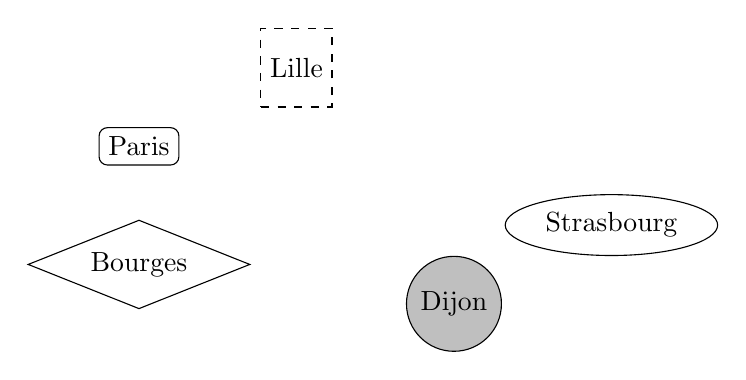
\begin{tikzpicture}
\node[draw,rectangle,rounded corners=3pt] (P)at(0,0){Paris};
\node[draw,minimum height=1cm,dashed] (L)at(2,1) {Lille};
\node[draw,ellipse] (S)at(6,-1) {Strasbourg};
\node[draw,diamond,aspect=2.5] (B)at(0,-1.5) {Bourges};
\node[draw,circle,fill=gray!50] (D)at(4,-2) {Dijon};
\end{tikzpicture}






\tikzstyle{ville}=[draw,rectangle,rounded corners=3pt]
\tikzstyle{capitale}=[draw,ellipse,very thick,fill=black!25]
\tikzset{ville/.style={draw,rectangle,rounded corners=3pt}}
\tikzset{capitale/.style={draw,ellipse,very thick,fill=black!25}}
\tikzset{radial/.style={very thick,->,>=stealth}}
\tikzset{transversal/.style={<->,>=stealth,thick,dashed}}
\begin{tikzpicture}
\node[capitale] (P)at(0,0){Paris};
\node[ville] (L)at(2,1){Lille};
\node[draw,ellipse] (S)at(6,-1) {Strasbourg};
\node[draw,diamond,aspect=2.5] (B)at(0,-1.5) {Bourges};
\node[draw,circle,fill=gray!50] (D)at(4,-2) {Dijon};
\draw[radial] (P)--(L);
\draw[transversal] (D)--(B);
\end{tikzpicture}









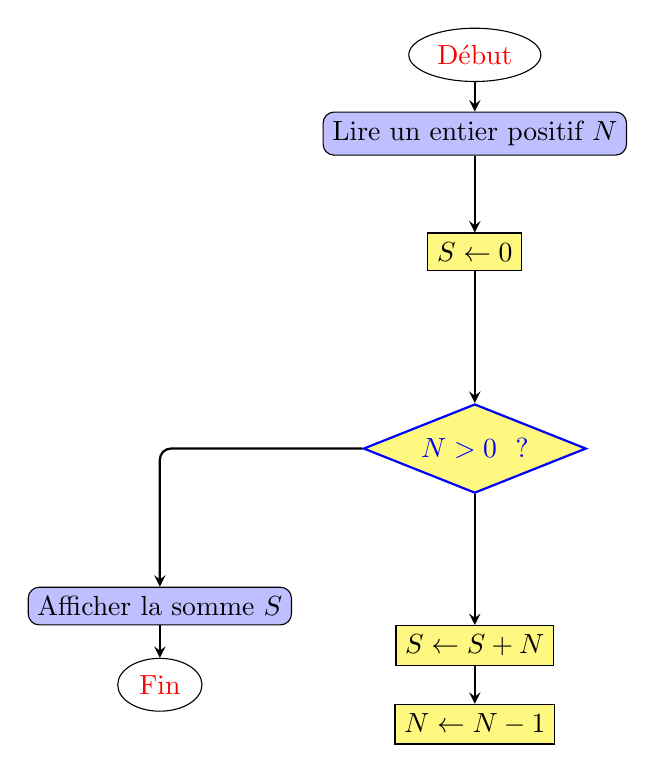
\begin{tikzpicture}
\tikzstyle{debutfin}=[ellipse,draw,text=red]
\tikzstyle{instruct}=[rectangle,draw,fill=yellow!50]
\tikzstyle{test}=[diamond, aspect=2.5,thick,
draw=blue,fill=yellow!50,text=blue]
\tikzstyle{es}=[rectangle,draw,rounded corners=4pt,fill=blue!25]

\node[debutfin] (debut) at (0,5) {Début};
\node[es] (lire) at (0,4) {Lire un entier positif $N$};
\node[test] (test) at (0,0) {$N>0$ \ ?};
\node[instruct] (init) at (0,2.5) {$S\leftarrow 0$};
\node[instruct] (plus) at (0,-2.5) {$S\leftarrow S+N$};
\node[instruct] (moins) at (0,-3.5) {$N\leftarrow N-1$};

\node[es] (afficher) at (-4,-2) {Afficher la somme $S$};
\node[debutfin] (fin) at (-4,-3) {Fin};

\tikzstyle{suite}=[->,>=stealth,thick,rounded corners=4pt]
\draw[suite] (debut) -- (lire);
\draw[suite] (lire) -- (init);
\draw[suite] (init) -- (test.north);
\draw[suite] (test) -- (plus);
\draw[suite] (plus) -- (moins);
\draw[suite] (test) -| (afficher);
\draw[suite] (afficher) -- (fin);

\end{tikzpicture}









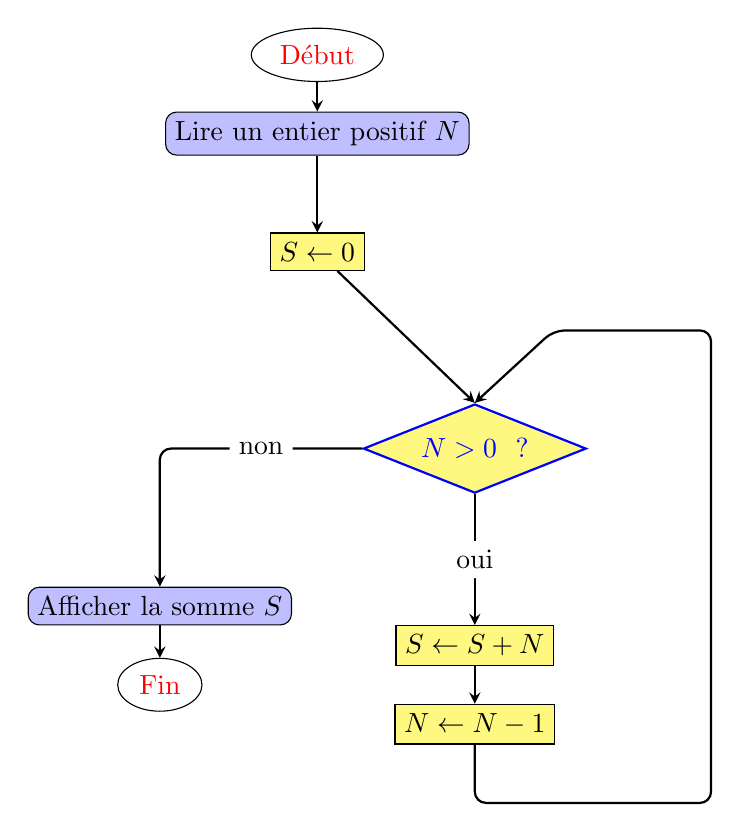
\begin{tikzpicture}
%styledesnœuds
\tikzstyle{debutfin}=[ellipse,draw,text=red]
\tikzstyle{instruct}=[rectangle,draw,fill=yellow!50]
\tikzstyle{test}=[diamond, aspect=2.5,thick,
draw=blue,fill=yellow!50,text=blue]
\tikzstyle{es}=[rectangle,draw,rounded corners=4pt,fill=blue!25]
%styledesflèches
\tikzstyle{suite}=[->,>=stealth,thick,rounded corners=4pt]
%placementdesnœuds
\node[debutfin] (debut) at (-2,5) {Début};
\node[es] (lire) at (-2,4) {Lire un entier positif $N$};
\node[test] (test) at (0,0) {$N>0$ \ ?};
\node[instruct] (init) at (-2,2.5) {$S\leftarrow 0$};
\node[instruct] (plus) at (0,-2.5) {$S\leftarrow S+N$};
\node[instruct] (moins) at (0,-3.5) {$N\leftarrow N-1$};
\node[es] (afficher) at (-4,-2) {Afficher la somme $S$};
\node[debutfin] (fin) at (-4,-3) {Fin};
%Placementdesflèches
\draw[suite] (debut) -- (lire);
\draw[suite] (lire) -- (init);
\draw[suite] (init) -- (test.north);
\draw[suite] (test) -- (plus) node[midway,fill=white]{oui};
\draw[suite] (plus) -- (moins);
\draw[suite] (moins)|-(3,-4.5) |- (1,1.5)--(test.north);
\draw[suite] (test)-|(afficher)node[near start,fill=white]{non};
\draw[suite] (afficher) -- (fin);
\end{tikzpicture}









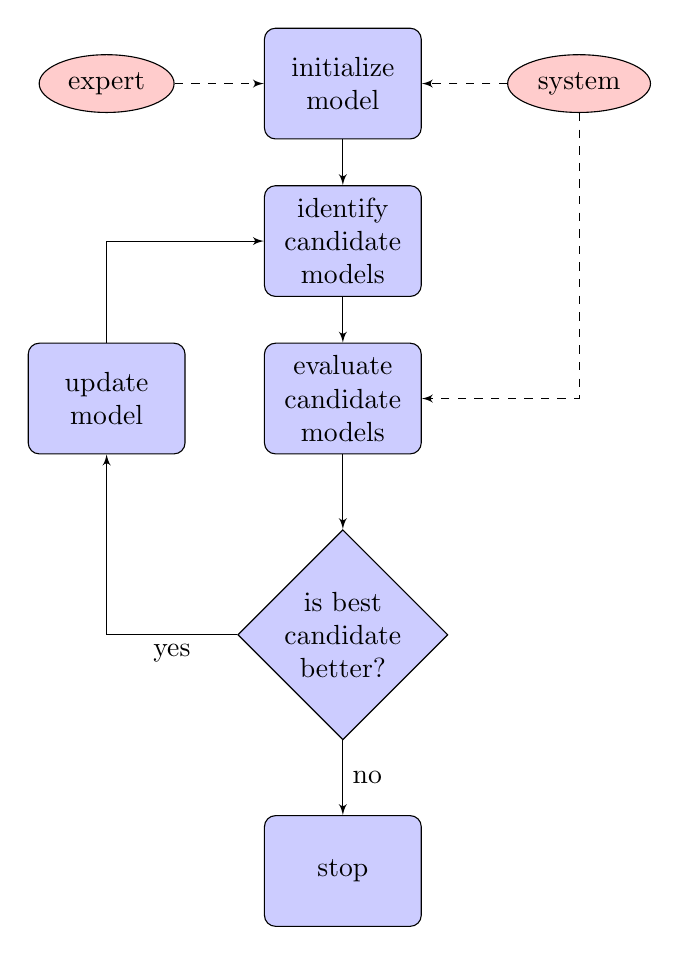
\begin{tikzpicture}[node distance = 2cm, auto]
	\tikzstyle{decision} = [diamond, draw, fill=blue!20, 
    text width=4.5em, text badly centered, node distance=3cm, inner sep=0pt]
\tikzstyle{block} = [rectangle, draw, fill=blue!20, 
    text width=5em, text centered, rounded corners, minimum height=4em]
\tikzstyle{line} = [draw, -latex']
\tikzstyle{cloud} = [draw, ellipse,fill=red!20, node distance=3cm,
    minimum height=2em]
    % Place nodes
    \node [block] (init) {initialize model};
    \node [cloud, left of=init] (expert) {expert};
    \node [cloud, right of=init] (system) {system};
    \node [block, below of=init] (identify) {identify candidate models};
    \node [block, below of=identify] (evaluate) {evaluate candidate models};
    \node [block, left of=evaluate, node distance=3cm] (update) {update model};
    \node [decision, below of=evaluate] (decide) {is best candidate better?};
    \node [block, below of=decide, node distance=3cm] (stop) {stop};
    % Draw edges
    \path [line] (init) -- (identify);
    \path [line] (identify) -- (evaluate);
    \path [line] (evaluate) -- (decide);
    \path [line] (decide) -| node [near start] {yes} (update);
    \path [line] (update) |- (identify);
    \path [line] (decide) -- node {no}(stop);
    \path [line,dashed] (expert) -- (init);
    \path [line,dashed] (system) -- (init);
    \path [line,dashed] (system) |- (evaluate);
\end{tikzpicture}










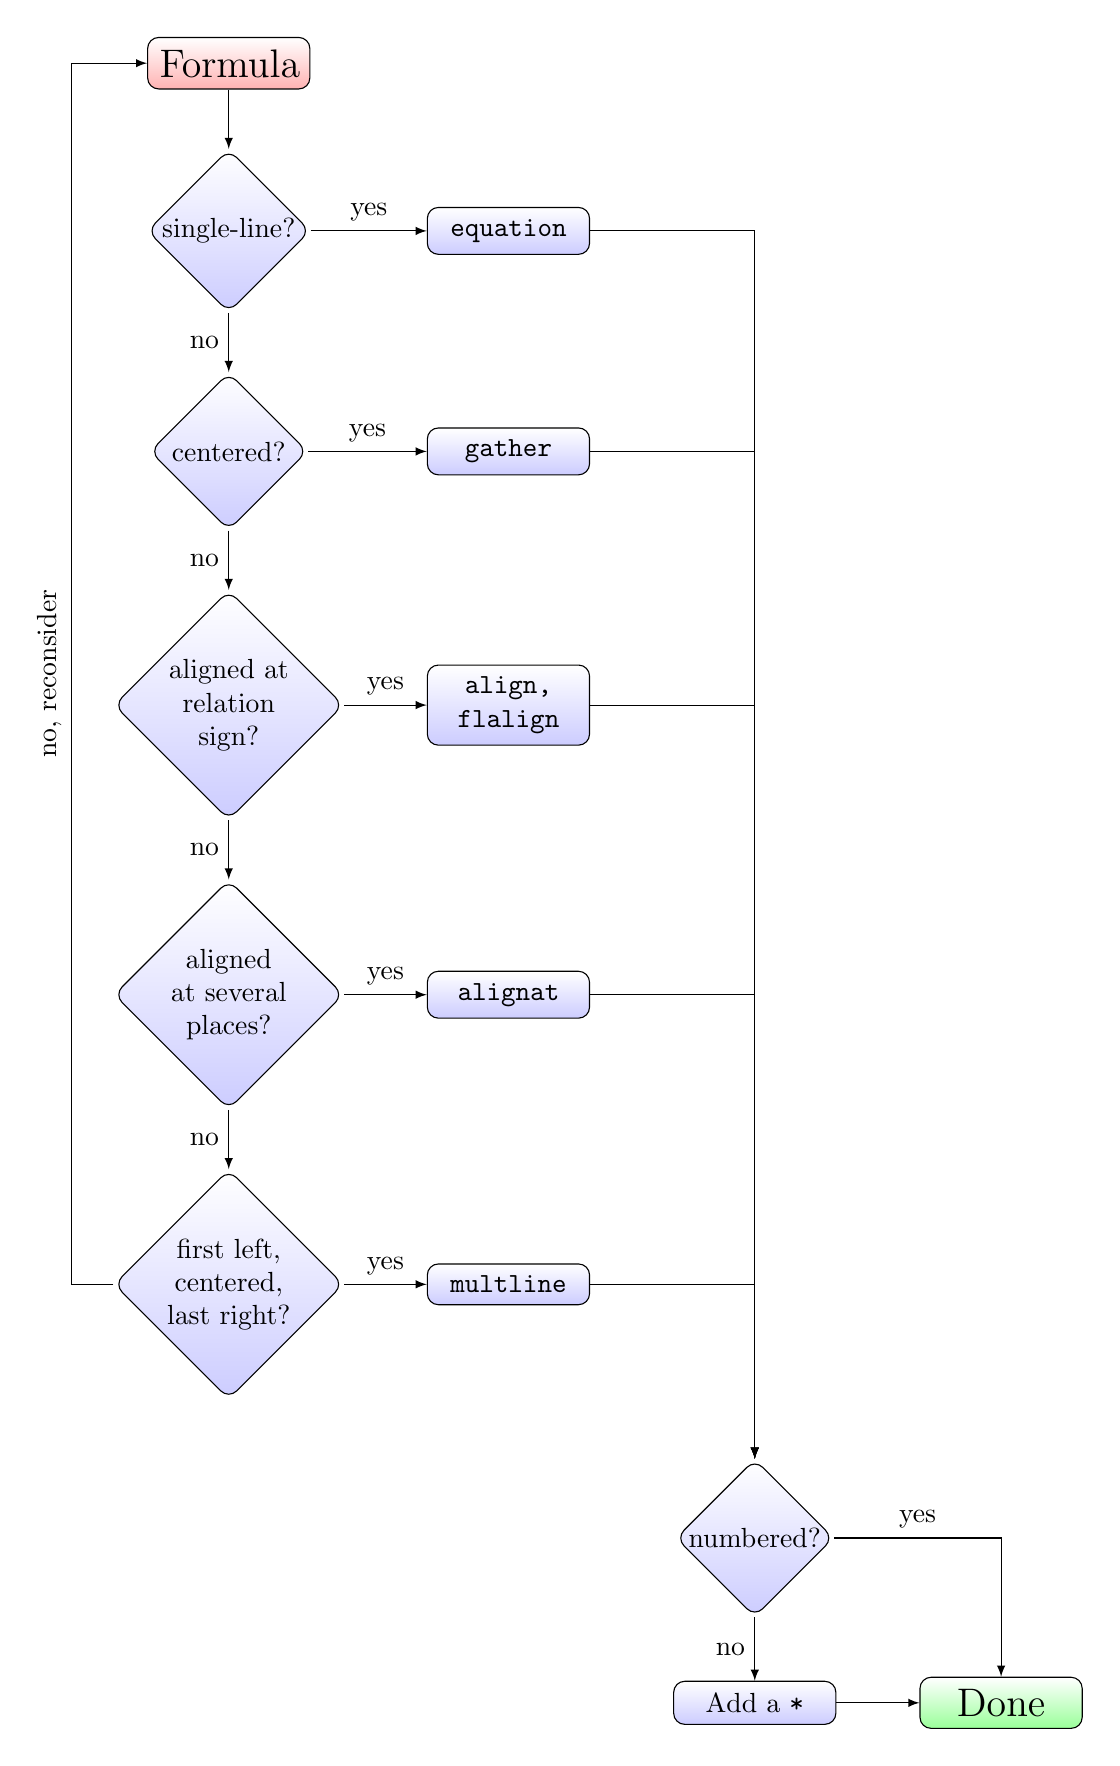
\begin{tikzpicture}[-latex]
\tikzset{
  treenode/.style = {shape=rectangle, rounded corners,
                     draw, anchor=center,
                     text width=5em, align=center,
                     top color=white, bottom color=blue!20,
                     inner sep=1ex},
  decision/.style = {treenode, diamond, inner sep=0pt},
  root/.style     = {treenode, font=\Large, bottom color=red!30},
  env/.style      = {treenode, font=\ttfamily\normalsize},
  finish/.style   = {root, bottom color=green!40},
  dummy/.style    = {circle,draw}
}
\newcommand{\yes}{edge node [above] {yes}}
\newcommand{\no}{edge  node [left]  {no}}
  \matrix (chart)
    [
      matrix of nodes,
      column sep      = 3em,
      row sep         = 5ex,
      column 1/.style = {nodes={decision}},
      column 2/.style = {nodes={env}}
    ]
    {
      |[root]| Formula           &                \\
      single-line?               & equation       \\
      centered?                  & gather         \\
      aligned at relation sign?  & align, flalign \\
      aligned at several places? & alignat        \\
      first left, centered,
        last right?              & multline       \\
      & & |[decision]| numbered? \\
      & & |[treenode]| Add a \texttt{*} & |[finish]| Done \\
    };
  \draw
    (chart-1-1) edge (chart-2-1)
    \foreach \x/\y in {2/3, 3/4, 4/5, 5/6} {
      (chart-\x-1) \no (chart-\y-1) }
    \foreach \x in {2,...,6} {
       (chart-\x-1) \yes (chart-\x-2) }
   (chart-7-3) \no  (chart-8-3)
   (chart-8-3) edge (chart-8-4);
 \draw
   (chart-6-1) -- +(-2,0) |- (chart-1-1)
     node[near start,sloped,above] {no, reconsider};
  \foreach \x in {2,...,6} {
   \draw (chart-\x-2) -| (chart-7-3);}
 \draw   (chart-7-3)  -| (chart-8-4)
   node[near start,above] {yes}; 
\end{tikzpicture}







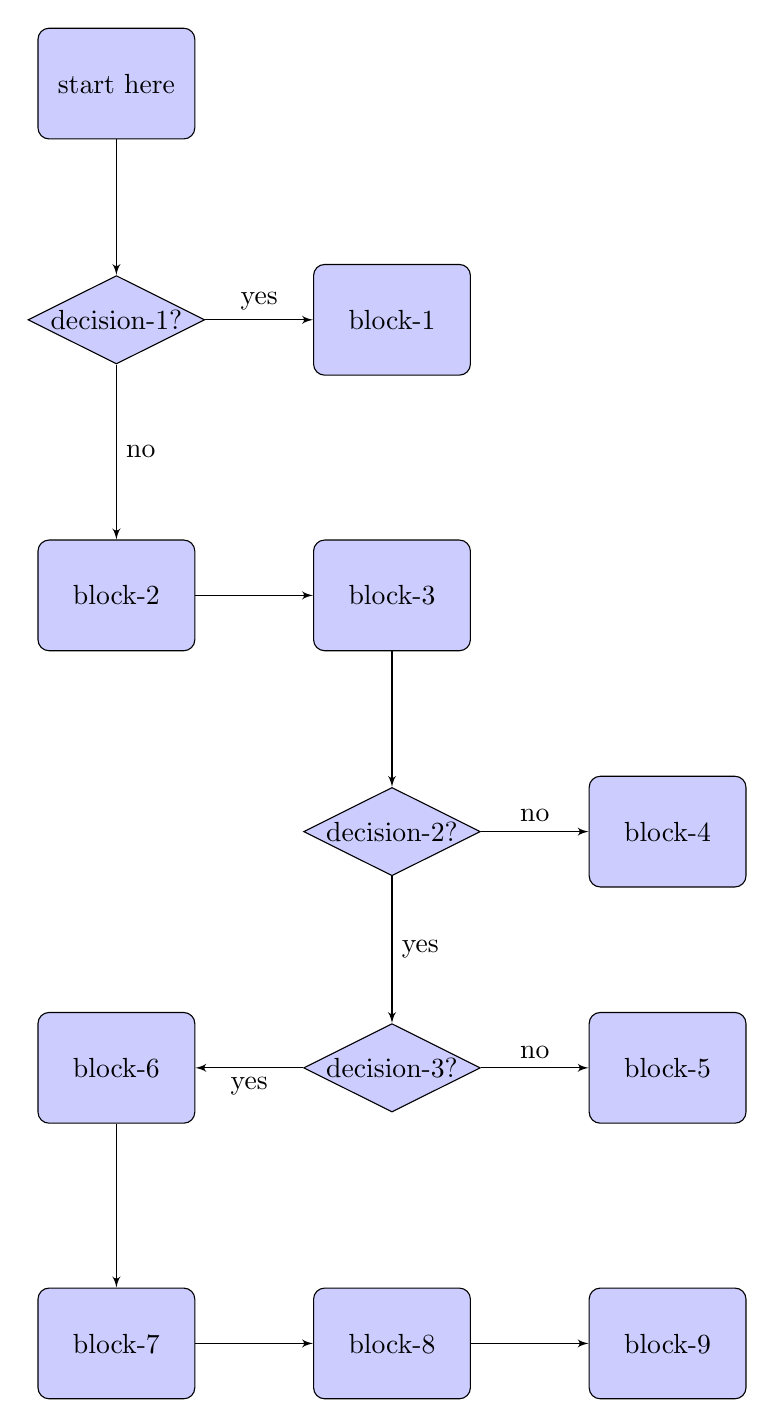
\begin{tikzpicture}[node distance=3.5cm, auto]
 \tikzstyle{decision} = [ diamond, aspect=2, draw, fill=blue!20, text width=5em, text badly centered, node distance=3cm, inner sep=0pt ]
\tikzstyle{block} = [ rectangle, draw, fill=blue!20, text width=5em, text centered, rounded corners, minimum height=4em ]
\tikzstyle{line} = [ draw, -latex' ]
% place nodes
\node [block] (init) {start here} ;
\node [decision, below of=init] (decision-1) {decision-1?} ;
\node [block, right of=decision-1] (block-1) {block-1} ;
\node [block, below of=decision-1] (block-2) {block-2} ;
\node [block, right of=block-2] (block-3) {block-3} ;
\node [decision, below of=block-3] (decision-2) {decision-2?} ;
\node [block, right of=decision-2] (block-4) {block-4} ;
\node [decision, below of=decision-2] (decision-3) {decision-3?} ;
\node [block, left of=decision-3] (block-6) {block-6} ;
\node [block, right of=decision-3] (block-5) {block-5} ;
\node [block, below of=block-6] (block-7) {block-7} ;
\node [block, right of=block-7] (block-8) {block-8} ;
\node [block, right of=block-8] (block-9) {block-9} ;


% draw edges
\path [line] (init) -- (decision-1) ;
\path [line] (decision-1) -- node {yes}(block-1) ;
\path [line] (decision-1) -- node {no}(block-2) ;
\path [line] (block-2) -- (block-3) ;
\path [line] (block-3) -- (decision-2) ;
\path [line] (decision-2) -- node {no}(block-4) ;
\path [line] (decision-2) -- node {yes}(decision-3) ;
\path [line] (decision-3) -- node {yes}(block-6) ;
\path [line] (decision-3) -- node {no}(block-5) ;
\path [line] (block-6) -- (block-7) ;
\path [line] (block-7) -- (block-8) ;
\path [line] (block-8) -- (block-9) ;
 
\end{tikzpicture}





\tikzstyle{block} = [rectangle, draw, fill=white, text width=6em, text centered, minimum height=5em]
\begin{tikzpicture}[node distance = 4cm, auto] \node [block] (sam) {Sample};
\node [block, right of=sam] (var) {Variable Selection};
\node [block, right of=var] (pro) {Data Colection/ Processing};
\node [block, right of=pro] (clu) {Clustering Algorithm Selection};
\node [block, below of=clu] (clus) {Clustering};
\node [block, left of=clus] (val) {Cluster Validation};
\node [block, left of=val] (res) {Result Interpretation}
\node [block, left of=res] (kno) {Knowledge};
\draw [->] (sam) -- (var);
\draw [->] (var) -- (pro);
\draw [->] (pro) -- (clu);
\draw [->] (clu) -- (clus);
\draw [->] (clus) -- (val);
\draw [->] (val) -- (res);
\draw [->] (res) -- (kno);
\end{tikzpicture}




\end{document}